\chapter{Bases}
The word "base" in mathematics is used to refer to a particular mathematical object that is used as a building block. The most common uses are the related concepts of the number system whose digits are used to represent numbers. In common, people use decimal system. However, the computers are compsed with binary system. Also, SHA-256 gives the hexadecimal code.
\section{Binary}
Binary is composed with only 0 and 1. Each of digits represents 2 to the power of something. From the right to left, it starts from $2^0$ to increasing the power.
	
\section{Decimals}
Decimal system is what people use in usual days. It is composed with 0,1,2,3,4,5,6,7,8, and 9, and it starts from $10^0$ and increases the power of 10 when it goes the next digit. The reason why people use the decimal system is that the human has 10 fingers, so the calculation is easier and more simple. 
\section{Hexadecimals}
Hexadecimal system is used for computer languages such as C language/C++ and SHA-256.It is composed with 1,2,3,4,5,6,7,8,9,a,b,c,d,e, and f. When the decimal numbers are hashed by SHA-256, it is more difficult if hashed number starts with 0 and have many 0s in the number. The number in front of x is the number of 0s which is leading.
\section{Conversion}
\begin{figure}
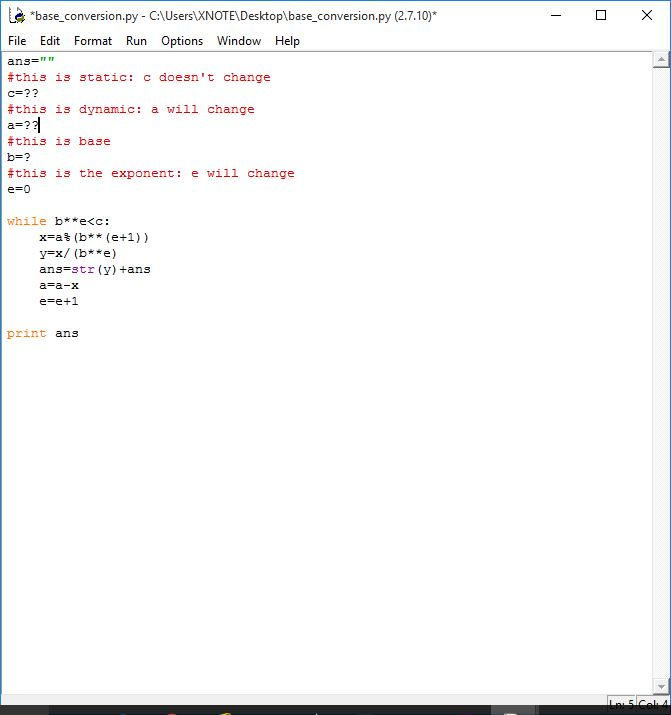
\includegraphics[width=10cm]{BaseConversion.jpg}
\end{figure}
It is the sample code of the base conversion. ? is what the base is, so it can be any decimal number. ?? can also be the any number, but decimal numbers. It changes from decimal numbers to base of ? numbers. a needs to be subtracted by x for the next step getting ? to the power of next exponent. Then, repeat the previous steps with e added 1. And then, repeat for next step again. At the last, however, y whicch is the quotient of the last x divided b to the power of e should be concantenated with ans. The quotient becomes the first number of the ? base numbers.
